\begin{figure*}[!ht]
  \centering
  \definecolor{barra}{HTML}{1F4E8C}
  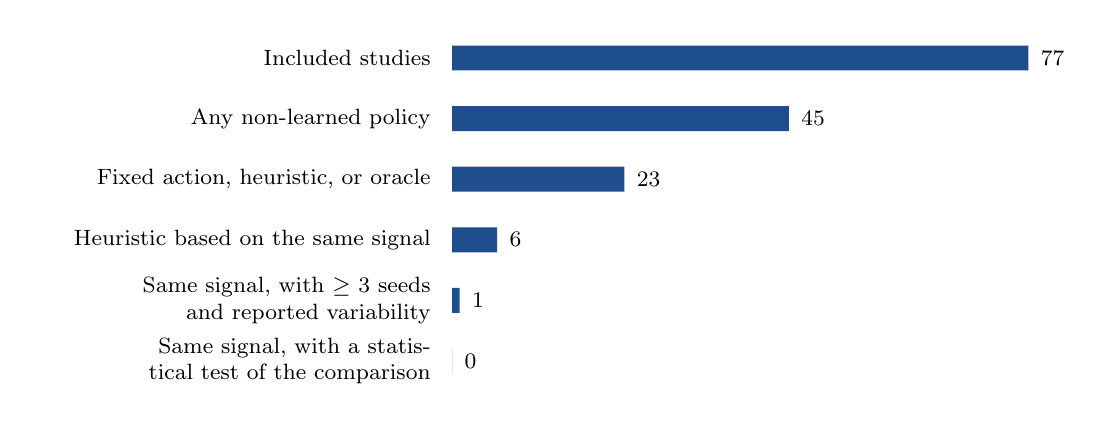
\begin{tikzpicture}
    \begin{axis}[
        xbar,
        bar width=9pt,
        width=0.82\linewidth,
        height=6.2cm,
        xmin=0, xmax=88,
        enlarge y limits=0.10,
        axis x line=none,
        axis y line*=left,
        y axis line style={draw=none},
        ytick style={draw=none},
        symbolic y coords={f,e,d,c,b,a},
        ytick={f,e,d,c,b,a},
        yticklabels={
          {Same signal, with a statistical test of the comparison},
          {Same signal, with $\geq$ 3 seeds and reported variability},
          {Heuristic based on the same signal},
          {Fixed action, heuristic, or oracle},
          {Any non-learned policy},
          {Included studies}
        },
        yticklabel style={
          font=\footnotesize,
          align=right,
          text width=5.0cm
        },
        nodes near coords,
        nodes near coords style={
          font=\footnotesize,
          anchor=west,
          text=black,
          xshift=1pt
        },
        clip=false
      ]
      \addplot[
        fill=barra,
        draw=none
      ] coordinates {
        (0,f)
        (1,e)
        (6,d)
        (23,c)
        (45,b)
        (77,a)
      };
    \end{axis}
  \end{tikzpicture}
  \caption{Evidence funnel for the incremental contribution of learning. Each stage contains unique studies and forms a subset of the preceding stage.}
  \label{fig:funil}
\end{figure*}
